%
% Latex Document made by TheInevitables for SRS,  COS 301 2017
%


\documentclass{article}

\usepackage{geometry}
\usepackage[utf8]{inputenc}
\usepackage{graphicx}
\usepackage{float}
\usepackage{amsmath}
\usepackage{amsfonts}
\usepackage{amssymb}
\usepackage{graphicx}
\usepackage{float}
\usepackage[explicit]{titlesec}
\usepackage{ulem}


\DeclareGraphicsExtensions{.png}
\DeclareGraphicsExtensions{.jpg}
\graphicspath{ {Diagrams/} }

 \geometry{
 a4paper, 
 total={170mm, 257mm}, 
 left=25mm, 
right=25mm, 
 top=25mm, 
 }
 
\begin{document}


\maketitle
\title 

\begin{figure}[h!]
\centering

\includegraphics[scale=0.5]{navLaunch.jpg}
\end{figure}

\author{
\center

    \author{The Inevitables: User Manual}
   
}

\newpage



\pagebreak
\tableofcontents
\pagebreak


\section{ User Manual}
\subsection{Installation}
To install the NavUP application you need to copy over the NavUP.apk file to your mobile device. On your mobile device file where you put the NavUP.apk file and double tap on it. your operating system should automatically try to install the NavUP application. Once the installation is complete you will find the application on you devices application menu.


\subsection{Login}
On startup of the application you will be presented with a login menu as shown below.

\begin{figure}[h!]
\centering
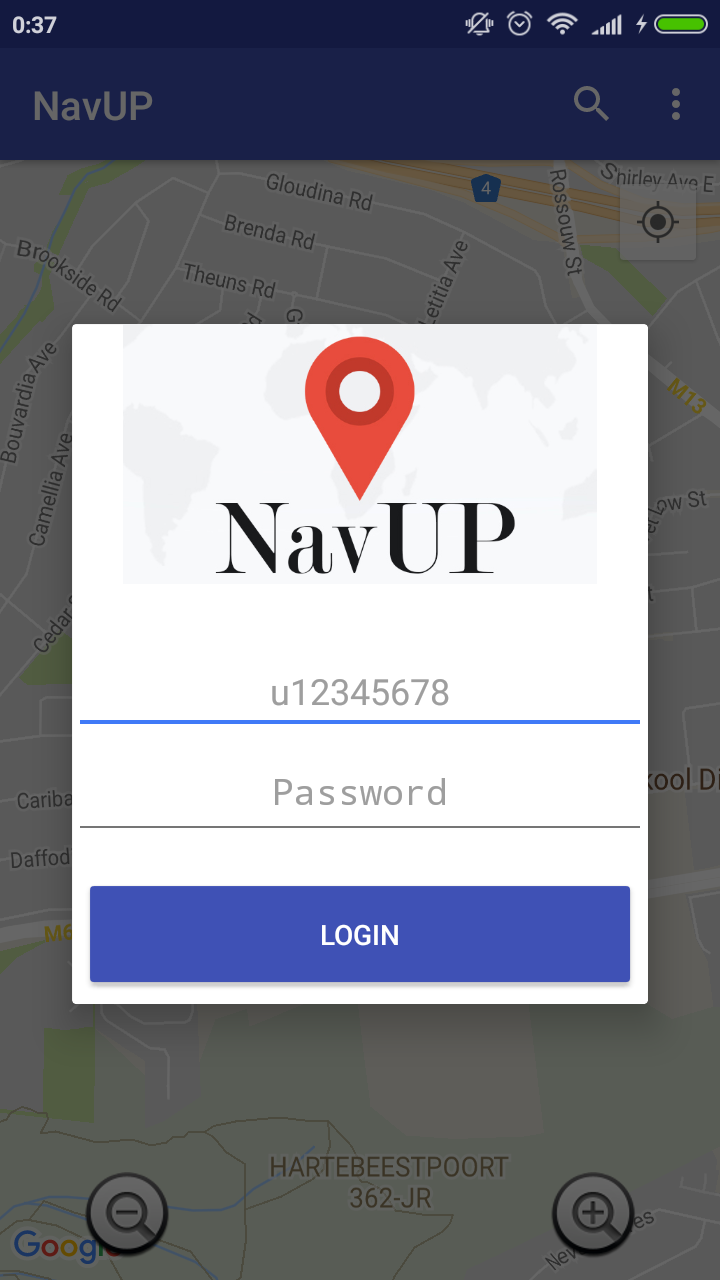
\includegraphics[scale=0.15]{login.png}
\end{figure}

Students are advised to login to ensure the latest information regarding their needs, those registered as students within the disability unit will automatically log into the disability unit app(this will provide extra features required by the disability unit). If you are a visitor simply click on the guest link ,this will allow you to continue using the application without logging in and provide basic navigation and may provide some extra information. 



\subsection{Main screen}
Once you have logged in you should see a screen like this.

\begin{figure}[h!]
\centering
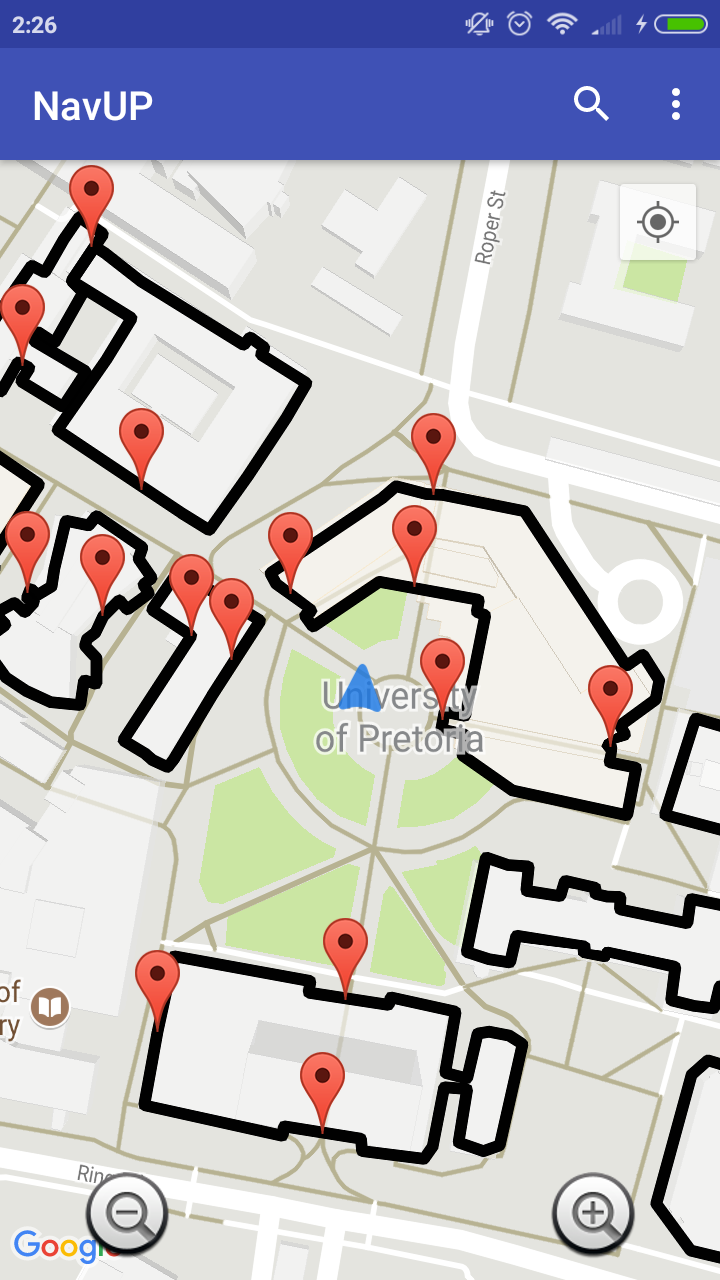
\includegraphics[scale=0.15]{topmap.png}
\end{figure}

The black outlines show the buildings on campus. These are able to be seen online and offline. In the center there is an arrow. This arrow is your current location. The red markers indicate entrances to the given buildings.
By taking two fingers to the screen and pushing up you can get a 3D model view of the area as shown below.

\newpage 

\begin{figure}[h!]
\centering
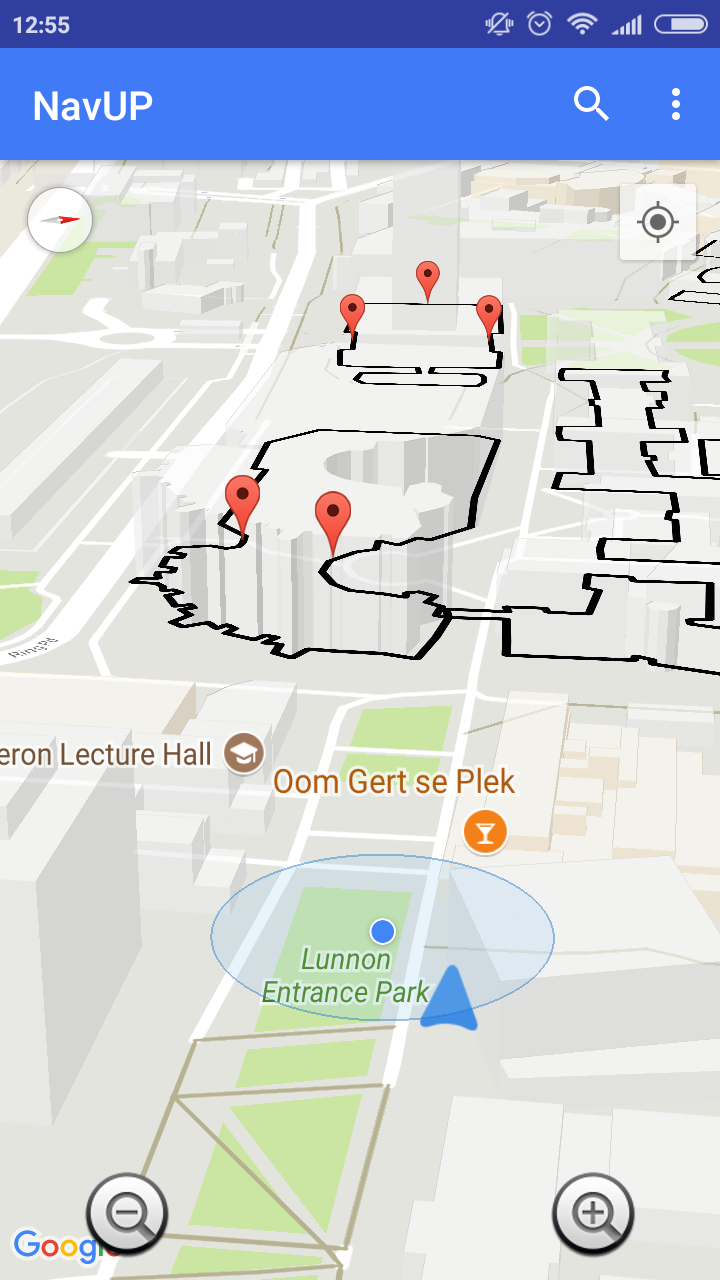
\includegraphics[scale=0.15]{3dmap.png}
\end{figure}

\subsection{Navigation}
To navigate enter the name of the building you would like to navigate too on the search bar at the top of the screen. 


\subsection{Menu}
The menu is on the top right hand corner and is a drop down menu. In this menu will be all the options that will be given to you based on the type of user you are. Disabled students will receive a menu different to those of other students. 

\subsection{Emergency Button}
The emergency button is only accessible to those who are logged in under a disability unit student number. The emergency button can be accessed from the menu and will send your current GPS coordinates to the administrator so that they can take the appropriate action that is needed.

\begin{figure}[h!]
\centering
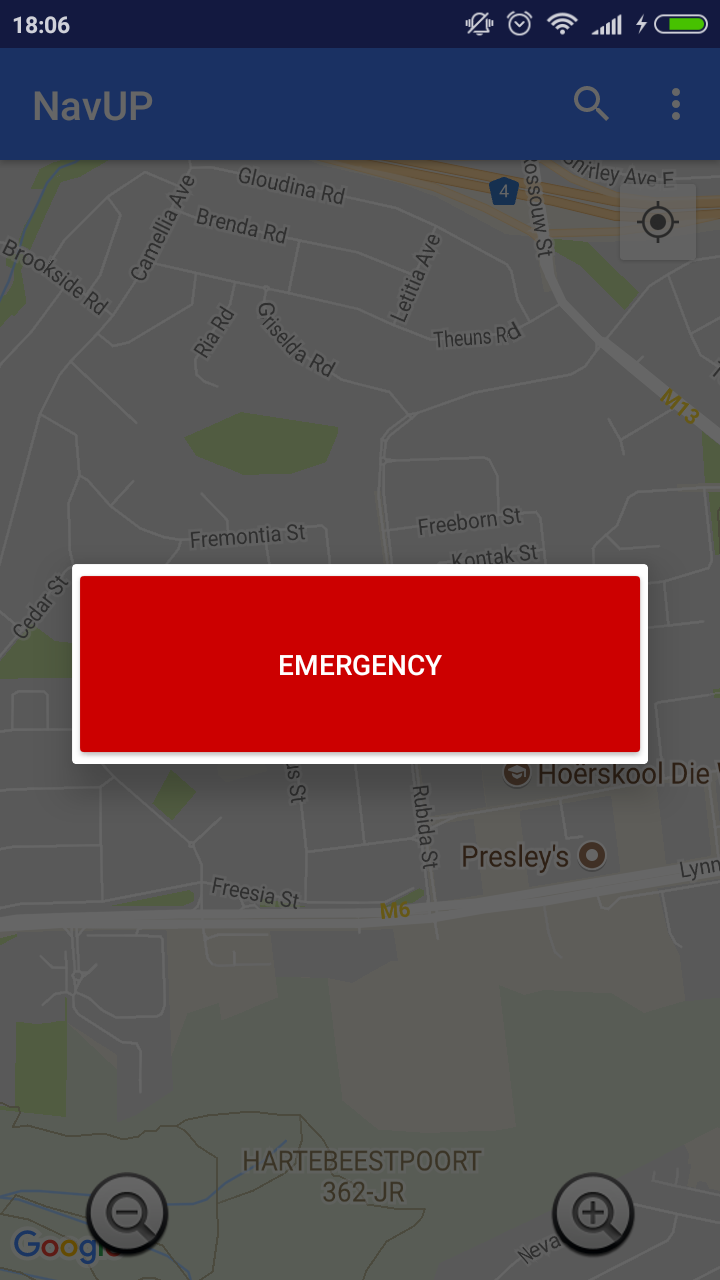
\includegraphics[scale=0.2]{emergency.png}
\end{figure}












\end{document}